\documentclass[tikz, border=10pt]{standalone}
\usepackage{pgfplots}
\pgfplotsset{compat=1.18}
\usetikzlibrary{calc}

\begin{document}

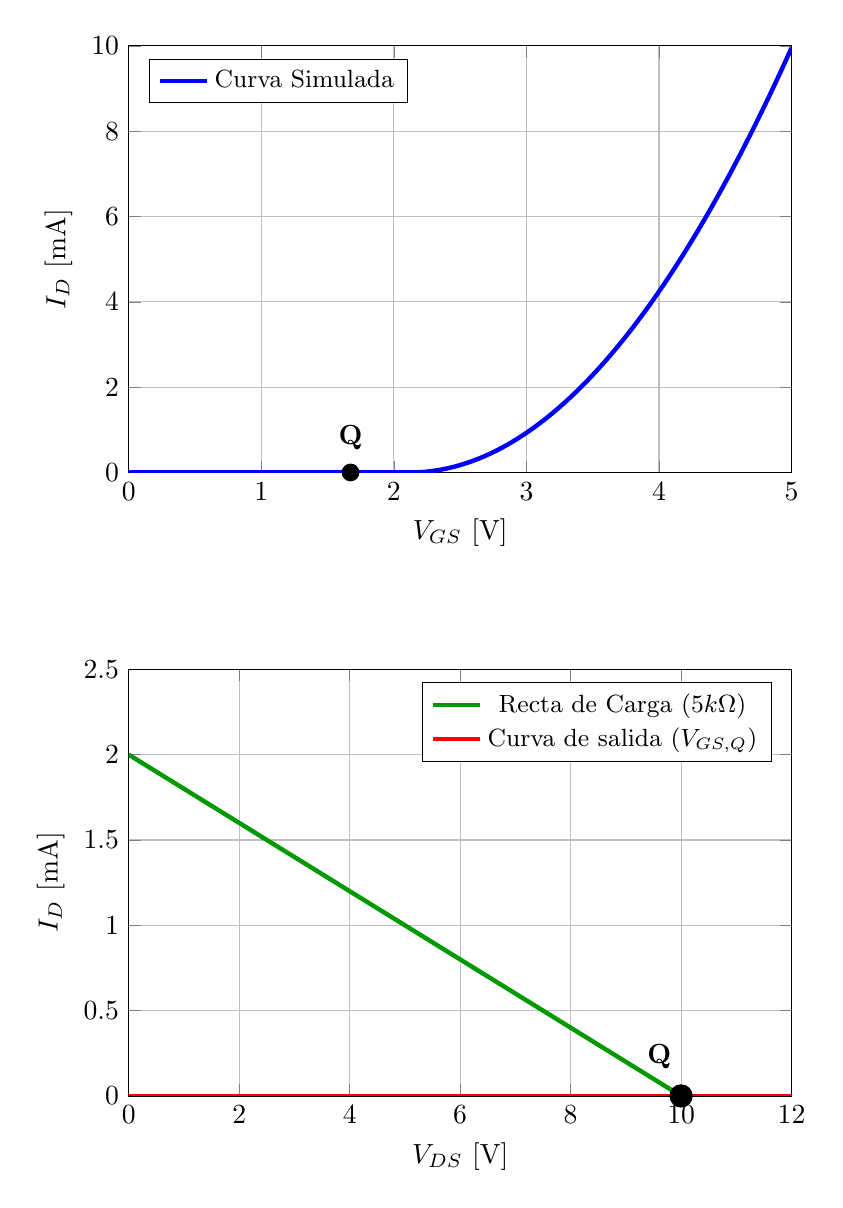
\begin{tikzpicture}
% --- GRÁFICO 1: ENTRADA (TRANSFERENCIA) ---
\begin{axis}[
    name=entrada,
    xlabel={$V_{GS}$ [V]},
    ylabel={$I_D$ [mA]},
    grid=both,
    width=10cm, height=7cm,
    xmin=0, xmax=5,
    ymin=0, ymax=10,
    legend pos=north west,
    legend style={font=\small}
]
    % Curva Simulada
    \addplot[blue, ultra thick, domain=2.12:5, samples=100] {1.2 * (x - 2.12)^2};
    \addplot[blue, ultra thick, domain=0:2.12] {0};
    \addlegendentry{Curva Simulada}

    % Punto Q de entrada
    \addplot[black, mark=*, mark size=3pt] coordinates {(1.673, 0)};
    \node[anchor=south] at (axis cs:1.673, 0.3) {\textbf{Q}};
\end{axis}

% --- GRÁFICO 2: SALIDA Y RECTA DE CARGA (SOLO INTERSECCIÓN) ---
\begin{axis}[
    name=salida,
    at={($(entrada.south)-(0,2.5cm)$)},
    anchor=north,
    xlabel={$V_{DS}$ [V]},
    ylabel={$I_D$ [mA]},
    grid=both,
    width=10cm, height=7cm,
    xmin=0, xmax=12,
    ymin=0, ymax=2.5,
    legend pos=north east,
    legend style={font=\small}
]
    % 1. Recta de Carga (10V / 5k)
    \addplot[green!60!black, ultra thick, domain=0:10] {(10 - x) / 5};
    \addlegendentry{Recta de Carga ($5k\Omega$)}
    
    % 2. Curva de salida correspondiente a Vgs = 1.673V (Corte)
    \addplot[red, ultra thick, domain=0:12] {0};
    \addlegendentry{Curva de salida ($V_{GS,Q}$)}
    
    % 3. PUNTO Q (Intersección: Recta de carga con Id=0)
    \addplot[black, mark=*, mark size=4pt] coordinates {(10, 0)};
    \node[anchor=south east] at (axis cs:10, 0.1) {\textbf{Q}};
\end{axis}
\end{tikzpicture}

\end{document}